%%%Pour afficher les réponses , activer l'option "answers" de la ligne documentclass
%Sans réponses
%\documentclass[twoside,a4paper,11pt]{exam}
%avec réponses
\documentclass[twoside,a4paper,11pt,answers]{exam}
\title{XX 1}
\date{}
\author{}


\usepackage{siunitx}
\usepackage{mystyles}
\usepackage[export]{adjustbox}
\usepackage{mathpazo}
\usepackage{booktabs}
\usepackage{framed}
\usepackage{listings}
\usepackage{mhchem}
\lstset
{upquote=true,
columns=flexible,
    basicstyle=\small\tt\hbox{}, 
	basicstyle=\ttfamily,
	language=Python,
    framesep=\fboxsep,
    framerule=\fboxrule,
    xleftmargin=\dimexpr\fboxsep+\fboxrule,
    xrightmargin=\dimexpr\fboxsep+\fboxrule,
	commentstyle=\color{gray},
	frame=single,
	rulecolor=\color{green!5},
	backgroundcolor=\color{gray!5},
	breaklines,
	numbers=left, 
	numbersep=5pt,  
	numberstyle=\scriptsize \ttfamily\color{gray},
	breakindent=1.5em,
	literate={Δ}{{$\mathtt{\Delta}$}}1 {‡}{{$\mathtt{\ddagger}$}}1
  {á}{{\'a}}1 {é}{{\'e}}1 {í}{{\'i}}1 {ó}{{\'o}}1 {ú}{{\'u}}1
  {Á}{{\'A}}1 {É}{{\'E}}1 {Í}{{\'I}}1 {Ó}{{\'O}}1 {Ú}{{\'U}}1
  {à}{{\`a~}}1 {è}{{\`e}}1 {ì}{{\`i}}1 {ò}{{\`o}}1 {ù}{{\`u}}1
  {À}{{\`A~}}1 {È}{{\'E}}1 {Ì}{{\`I}}1 {Ò}{{\`O}}1 {Ù}{{\`U}}1
  {ä}{{\"a}}1 {ë}{{\"e}}1 {ï}{{\"i}}1 {ö}{{\"o}}1 {ü}{{\"u}}1
  {Ä}{{\"A}}1 {Ë}{{\"E}}1 {Ï}{{\"I}}1 {Ö}{{\"O}}1 {Ü}{{\"U}}1
  {â}{{\^a}}1 {ê}{{\^e}}1 {î}{{\^i}}1 {ô}{{\^o}}1 {û}{{\^u}}1
  {Â}{{\^A}}1 {Ê}{{\^E}}1 {Î}{{\^I}}1 {Ô}{{\^O}}1 {Û}{{\^U}}1
  {œ}{{\oe}}1 {Œ}{{\OE}}1 {æ}{{\ae}}1 {Æ}{{\AE}}1 {ß}{{\ss}}1
  {ç}{{\c c}}1 {Ç}{{\c C}}1 {ø}{{\o}}1 {å}{{\r a}}1 {Å}{{\r A}}1
  {€}{{\EUR}}1 {£}{{\pounds}}1 {×}{{$\times$}}1,       
}



\begin{document}

\section{Suivi cinétique de la mutarotation du glucose}

Le D-glucose est une molécule naturelle appartenant à la famille des sucres, de formule brute \ce{C6H12O6} et de formule topologique ci-dessous :

\begin{center}
    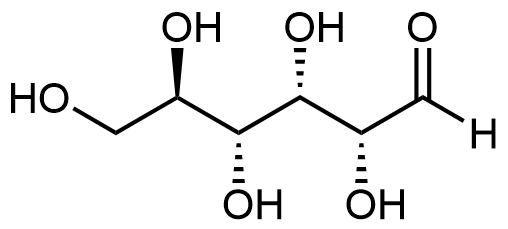
\includegraphics[scale = 0.3]{images/glucose_lineaire.png}
    \captionof{figure}{Forme linéaire du D-Glucose}
\end{center}

En vérité le glucose est plutôt sous forme cyclique, obtenue à partir de la forme linéaire selon un mécanisme d'hémiacétalisation. Il existe deux diastéréoisomères, l'$\alpha$-D-glucose et le $\beta$-D-glucose. En solution aqueuse, il s'établit un équilibre entre ces deux diastéréoisomères, c'est la \textbf{mutarotation}. On a alors environ 36\% de forme $\alpha$ et 64\% de forme $\beta$ à 25°C.

\begin{center}
    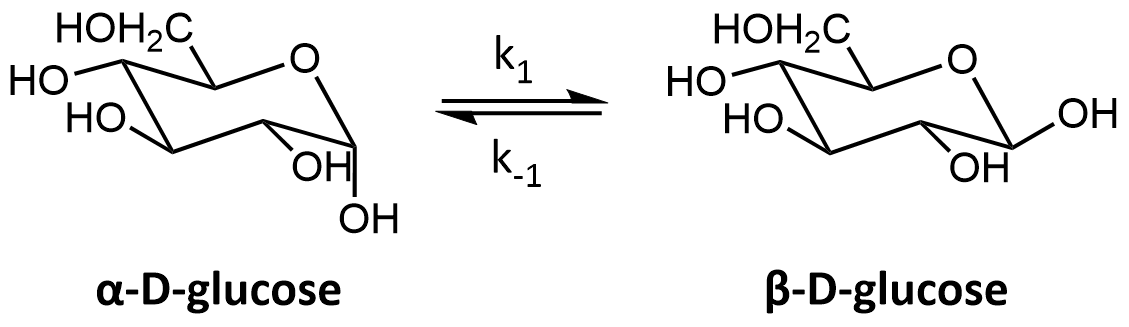
\includegraphics[scale = 0.3]{images/mutarotation.png}
    \captionof{figure}{Mutarotation entre les formes cycliques du glucose}
\end{center}


Nous allons nous intéresser au suivi cinétique de cette réaction. On note $x_{0}$ la fraction molaire en $\alpha$-D-glucose, $y$ l'avancement à l'instant t de la réaction dans le sens de la transformation en le diastéréoisomère $\beta$. En considérant les processus dans le sens 1 et -1, et en supposant un ordre 1 par rapport à chacune des formes du glucose, on peut montrer la relation suivante : 

\begin{equation}
    \frac{dy}{dt} = (k_1 + k_{-1})(y_{\infty} - y)
    \label{eq:vitesse}
\end{equation}

où $y_{\infty}$ est l'avancement à l'équilibre.

\begin{questions}
\begin{framed}
\question Démontrer la relation \ref{eq:vitesse}.
\begin{solution}[6cm]
\begin{flushleft}
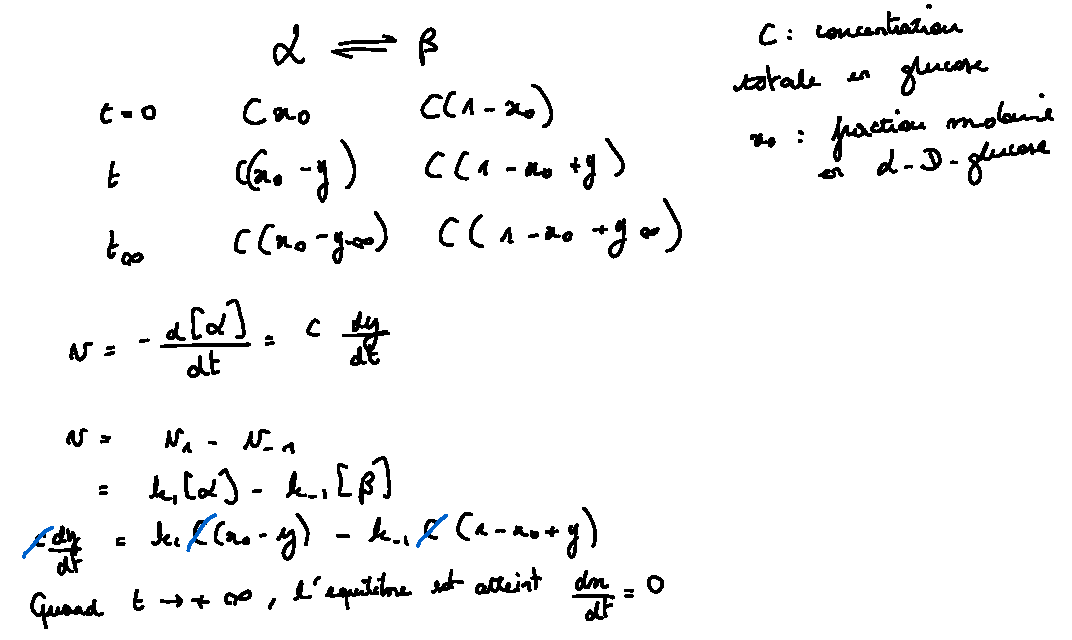
\includegraphics[scale = 0.8]{images/demo_muta_1.pdf}
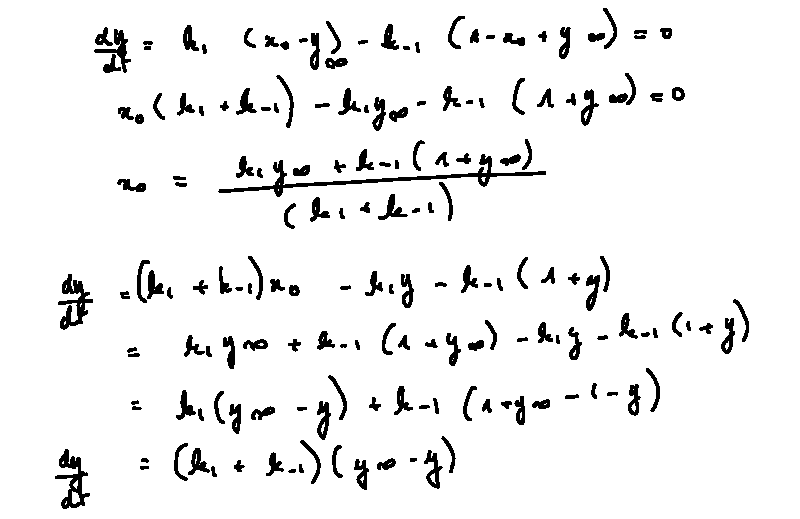
\includegraphics[scale = 0.8]{images/demo_muta_2.pdf}
\end{flushleft}
\end{solution}
\end{framed}


\begin{framed}
\question Pourquoi est-il pertinent dans ce cas de proposer un ordre 1 par rapport aux deux formes ?
\begin{solution}[1cm]
Car il s'agit d'une réaction monomoléculaire.
\end{solution}
\end{framed}



L'équation \ref{eq:vitesse} peut être intégrée pour donner l'équation suivante :
\begin{equation}
    \ln{\frac{y_{\infty} - y}{y_{\infty}}} = -(k_1 + k_{-1})t
    \label{eq:integree}
\end{equation}

On peut alors exprimer l'avancement en fonction du pouvoir rotatoire et on obtient l'équation :

\begin{equation}
    \ln{\frac{\alpha - \alpha_{\infty}}{\alpha_0 - \alpha_{\infty}}} = -(k_1 + k_{-1})t
\end{equation}

Où $\alpha_0$ est le pouvoir rotatoire initial de la solution de glucose, juste après la dissolution.



\par Cette réaction peut être accélérée sous catalyse acido-basique. La constante $k_1 + k_{-1}$ dépend alors de la concentration en catalyseur.

~

\paragraph{Catalyse acido-basique spécifique ou généralisée}

~

\par Dans certains cas de catalyse acido-basique, la vitesse de la réaction dépend de la concentration de toute espèce acide ou basique présente en solution. On parle alors de catalyse acido-basique \emph{généralisée}. Dans d'autres cas la vitesse dépend simplement de la concentration en ions hydronium \ce{H+} ou hydroxyde \ce{HO-} présents en solution, c'est à dire du pH. On parle alors de catalyse acido-basique \emph{spécifique}.

~

\par Dans le cas de la mutarotation du glucose, on a alors deux expressions possibles pour la valeur de la constante $k_1 + k_{-1}$.
\begin{itemize}
    \item catalyse acido-basique \emph{spécifique} : $k_1 + k_{-1} = k_0\con{\ce{H3O+}} +  + k'$
    \item catalyse acido-basique \emph{généralisée}  : $k_1 + k_{-1} = k_0\con{\ce{H3O+}} + \sum_{i=1}^{n} k_i \con{HA_i} + k'$
\end{itemize}

~

\par On utilise deux solutions pour préparer le milieu dans lequel va être étudiée la mutarotation du glucose :
\begin{itemize}
    \item une solution tampon \textbf{A} constituée d'un mélange d'ions dihydrogénophosphate \ce{H2PO4-} et hydrogénophosphate \ce{HPO4^{2-}}, chacun à la concentration de 0,10 \unit{\mol.\liter^{-1}} ;
    \item une solution ionique \textbf{B} constituée de chlorure de sodium \ce{NaCl} à 0,40 \unit{\mol.\liter^{-1}}.
\end{itemize} 

~

\par La solution tampon \textbf{A} peut être diluée, mais afin de maintenir son pouvoir tampon, il faut que la concentration totale en ions soit constante, c'est pourquoi on utilise la solution \textbf{B}.

~

\par \textbf{Préparer 100 mL de la solution B}.
\begin{solution}
    Il suffit de dissoudre 2,33g de \ce{NaCl} dans une fiole de 100 mL avec de l'eau distillée.
\end{solution}

~





\par Le suivi cinétique par polarimétrie (cuve de longueur 20 cm) de la mutarotation du glucose dans une solution obtenue par dissolution de 10g de glucose dans 12,5 mL de solution \textbf{A} et 37,5 mL de solution \textbf{B} a donné une mesure de la constante $k_1 + k_{-1}$ de $1,342.10^{-3} \unit{s^{-1}}$.



\begin{framed}
\question Calculer la concentration en espèce acido-basique du phosphore dans ces conditions.
\begin{solution}[1cm]
    concentration totale en phosphore = $\con{\ce{H2PO4-}} + \con{\ce{HPO4-}} = 2\cdot \frac{0.10 \cdot 12,5}{37,5+12,5} = 0,5  \unit{\mol\per\liter}$ 
\end{solution}
\end{framed}

\begin{framed}
\question En admettant que le volume de solution obtenu par dissolution de 10g de glucose dans 50 mL de solution vaut 55 mL, calculer la valeur attendue du pouvoir rotatoire à l'équilibre, $\alpha_{\infty}$.
\begin{solution}[3cm]
En négligeant la variation de volume par ajout de glucose on a une concentration totale en glucose $C_{glu} = \frac{10}{55.10^{-3}} = 1,8.10^{2} \unit{g.mL^{-1}}$. En admettant qu'à l'équilibre on ait 36\% de diastéréosimoère $\alpha$ et 64\% de diastéréosisomère $\beta$, $\alpha_{infty} = ([\alpha]_{\alpha} \cdot 0,36 + [\alpha]_{\beta} \cdot 0,64) \cdot 2 \cdot C_{glu} = (112 \cdot 0,36 + 19 \cdot 0,64) \cdot 2 \cdot 0,18 = 18,9 \unit{\degree}$
\end{solution}
\end{framed}


\begin{center}
    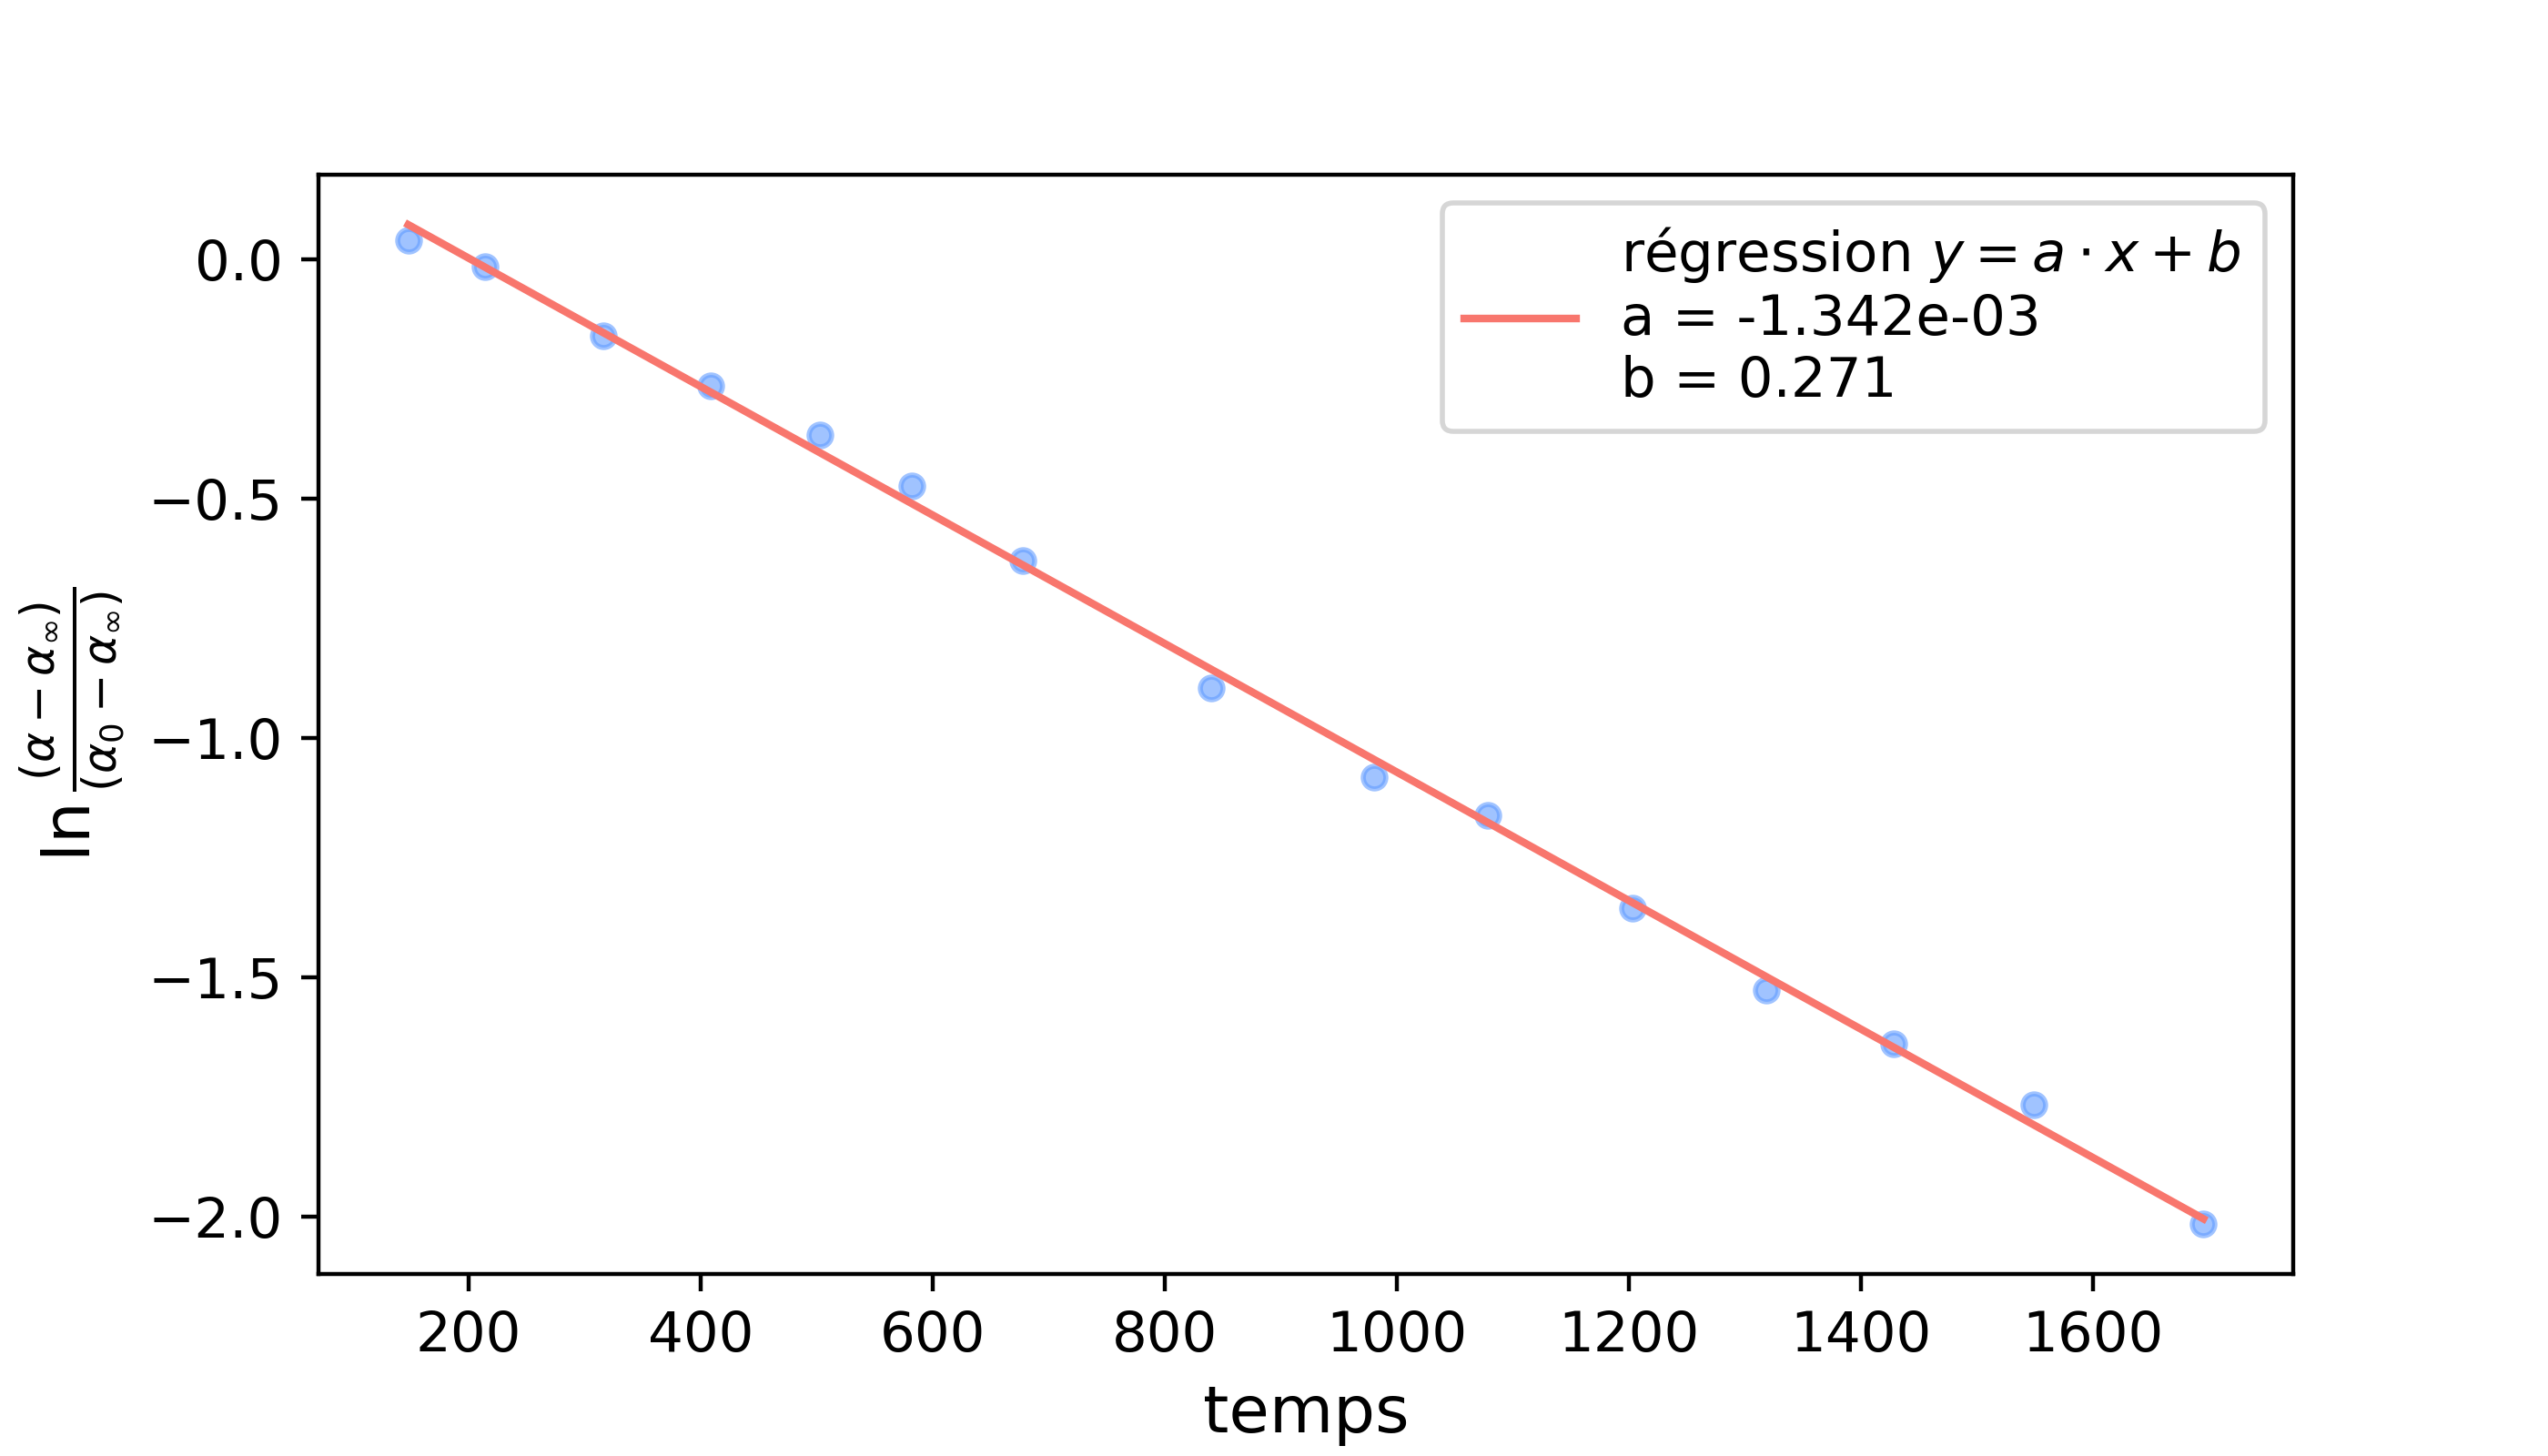
\includegraphics[width = 14cm]{images/suivi_glucose.png}
    \captionof{figure}{Suivi cinétique de la mutarotation du glucose dans 12,5 mL de solution \textbf{A} et 37,5 mL de solution \textbf{B}}
\end{center}
~


\par \textbf{Proposer un protocole qui permette de conclure quant au caractère acido-basique spécifique ou généralisé de la catalyse de la mutarotation du glucose.}

\begin{solution}
    En faisant différents suivis à pH constant mais imposé par des concentrations différentes en tampon on peut montrer qu'il s'agit d'une catalyse spécifique si la pente $k_1 + k_{-1}$ est identique dans toutes les expériences (le pH est constant) ou généralisée si elle varie avec la concentration du tampon. Comme la cinétique est assez longue (environ 30 minutes), on considérera qu'un seul autre suivi où on trouve une valeur de constante $k_1 + k_{-1}$ est suffisant. On peut faire une solution deux fois plus concentrée en tampon en mélangeant 25 mL de \textbf{A} et 25 mL de \textbf{B}. Pour avoir la dissolution la plus rapide, il est important de verser la solution dans un bécher, de lancer l'agitation, puis d'ajouter les 10g de glucose sous agitation vigoureuse en lançant le chronomètre. Une fois la dissolution terminée, il faut remplir la cuve de polarimétrie rapidement et faire des mesures toutes les minutes environ. Une première mesure devrait pouvoir être faite entre une et deux minutes après le début de la réaction. La cuve polarimétrique peut être laissée dans le polarimètre pour avoir la valeur de $\alpha_{infty}$ au delà de 30 minutes. On trace ensuite $\ln{\frac{\alpha - \alpha_{\infty}}{\alpha_0 - \alpha_{\infty}}}$ en fonction du temps et on détermine l'opposé de la pente par regression linéaire. Attention, les valeurs finales prcohes de $\alpha_{\infty}$ ne doivent pas être prises en compte car le logarithme diverge.
\end{solution}

\par \textit{Mettre en oeuvre votre protocole expérimental après validation par un examinateur.}

\begin{framed}
\question Comment estimer l'incertitude sur le pouvoir rotatoire mesuré ?
\begin{solution}[3cm]

\end{solution}
\end{framed}


\end{questions}

\paragraph*{Pouvoirs rotatoires spécifiques des formes cycliques du glucose} :
\begin{itemize}
        \item Pour l'$\alpha$-D-glucose : $[\alpha]_{\alpha}$ = 112 \unit{\degree.g^{-1}.mL.dm^{-1}} 
        \item Pour le $\beta$-D-glucose : $[\alpha]_{\beta}$ = 19 \unit{\degree.g^{-1}.mL.dm^{-1}} 
\end{itemize}

\end{document}